\section*{Multiple-choice}\label{sec:mc}

Dine svar skal indtastes i ITX-systemets multiple-choice modul.

\multiplechoicestart

\spoergsmaal{Rekursionsligninger}
Antag at $T_i(n)=1$ for $n \leq 1$ for $i=1,\dots,6$. Hvilke af følgende påstande om løsningen til en rekursionsligning er sande?
\fleresvar
\mulighederstart
\svar $T_1(n) = 2\cdot T_1(n/2) + \Theta(n)$ har løsningen $T_1(n) = \Theta(n \log n)$. \korrekt
\svar $T_2(n) = T_2(n/4) + \Theta(n)$ har løsningen $T_2(n) = \Theta(n)$. \korrekt
\svar $T_3(n) = 3\cdot T_3(n/3) + \Theta(n \log n)$ har løsningen $T_3(n) = \Theta(n \log^2 n)$. \korrekt
\svar $T_4(n) = 7\cdot T_4(n/2) + \Theta(n^2)$ har løsningen $T_4(n) = \Theta(n^3)$.
\svar $T_5(n) = T_5(n-1) + \Theta(\log n)$ har løsningen $T_5(n) = \Theta(\log^2 n)$.
\svar $T_6(n) = 4\cdot T_6(n/2) + \Theta(n \log n)$ har løsningen $T_6(n) = \Theta(n^2)$. \korrekt
\mulighederslut

\forklaring{
$T_1$: Master theorem med $a=2$, $b=2$, $f(n)=\Theta(n)$ giver $\Theta(n \log n)$.
$T_2$: $a=1$, $b=4$, $f(n)=\Theta(n) = \Omega(n^{\log_b a + \varepsilon})$, så løsning er $\Theta(n)$.
$T_3$: Master theorem tilfælde 2 (grænsetilfælde), $a=3$, $b=3$, $f(n)=\Theta(n \log n)$ giver $\Theta(n \log^2 n)$.
$T_4$: $a=7$, $b=2$, $f(n)=\Theta(n^2)$; da $n^{\log_b a} = n^{\log_2 7}$, og $f(n)$ vokser langsommere, gives løsning $\Theta(n^{\log_2 7})$.
$T_5$: Ved induktion kan ses at løsningen er summen af $\log i$ for $i=1$ til $n$, hvilket er $\Theta(n \log n)$, ikke $\log^2 n$.
$T_6$: $a=4$, $b=2$, $f(n)=\Theta(n \log n)$ og $n^{\log_b a} = n^2$; da $f(n) = o(n^2)$, bruges master theorem tilfælde 1 og giver $\Theta(n^2)$.
}


\spoergsmaal{Merge-Sort variant}
Betragt en variant af {\sc Merge-Sort} der deler input op i fire dele, hver af størrelse omtrent $n/4$, sorterer dem rekursivt, og fletter de fire sorterede delmængder sammen med tre kald til {\sc Merge} (fra CLRS sektion 2.3). Pseudokoden er:

{\small\begin{codebox}
  \Procname{$\proc{Merge4-Sort}(A, p, s)$}
  \li \If $p<s$ \Do
  \li $q_1 = \lfloor (3p+s)/4\rfloor$
  \li $q_2 = \lfloor (p+s)/2\rfloor$
  \li $q_3 = \lfloor (p+3s)/4\rfloor$
  \li $\proc{Merge4-Sort}(A, p, q_1)$
  \li $\proc{Merge4-Sort}(A, q_1+1, q_2)$
  \li $\proc{Merge4-Sort}(A, q_2+1, q_3)$
  \li $\proc{Merge4-Sort}(A, q_3+1, s)$
  \li $\proc{Merge}(A, p, q_1, q_2)$
  \li $\proc{Merge}(A, p, q_2, q_3)$
  \li $\proc{Merge}(A, p, q_3, s)$ \End
\end{codebox}}

\noindent
Hvilken rekursionsligning beskriver køretiden $T(n)$ for $\proc{Merge4-Sort}$ på et input af størrelse $n$ (hvor $n=s-p+1$)?
\etsvar
\mulighederstart
\svar $T(n) = 3\cdot T(n/4) + \Theta(n)$
\svar $T(n) = 3\cdot T(n/4) + \Theta(n\lg n)$
\svar $T(n) = 3\cdot T(n/4) + \Theta(n^2)$
\svar $T(n) = 4\cdot T(n/4) + \Theta(n)$ \korrekt
\svar $T(n) = 4\cdot T(n/4) + \Theta(n\lg n)$
\svar $T(n) = 4\cdot T(n/4) + \Theta(n^2)$
\mulighederslut
\forklaring{De fire rekursive kald kører på inputstørrelser på ca.~$n/4$, og andre operationer inkl.~de tre fletningskald tager samlet $\Theta(n)$ tid. Dermed gælder $T(n)=4\cdot T(n/4)+\Theta(n)$.}

\spoergsmaal{Tumpesortering}
Betragt denne algoritme, der tager et array $A[1:n]$ og to indekser $i,j$ som input, hvor $i\leq j$.
Det kan vises at $A$ bliver sorteret af kaldet $\proc{Tumpesortering}(A, 1, n)$.
\begin{codebox}
\Procname{$\proc{Tumpesortering}(A, i, j)$}
\li \If $A[i] > A[j]$ \Then
\li     swap $A[i]$ with $A[j]$
    \End
\li \If $j \geq i + 2$ \Then
\li     $t = \lfloor (j - i + 1) / 3 \rfloor$
\li     $\proc{Tumpesortering}(A, i, j - t)$
\li     $\proc{Tumpesortering}(A, i + t, j)$
\li     $\proc{Tumpesortering}(A, i, j - t)$
    \End
\end{codebox}
Lad $T(n)$ være køretiden af kaldet $\proc{Tumpesortering}(A, 1, n)$, hvor $A$ er et array af længde $n$.
Hvilke af følgende udsagn gælder for $T(n)$?
\fleresvar
\mulighederstart
\svar Køretiden kan beskrives ved rekursionen
\[
T(n) =
\begin{cases} 
\Theta(1), & \text{for } n = 1 \\
3\,T(n-1) + \Theta(1), & \text{for } n > 1.
\end{cases}
\]
\itxsvar{T(n) = 3T(n-1) + Theta(1)}
\svar Køretiden kan beskrives ved rekursionen
\[
T(n) =
\begin{cases} 
\Theta(1), & \text{for } n = 1 \\
3\,T(n/3) + \Theta(1), & \text{for } n > 1.
\end{cases}
\]
\itxsvar{T(n) = 3T(n/3) + Theta(1)}
\svar Køretiden kan beskrives ved rekursionen \korrekt
\[
T(n) =
\begin{cases} 
\Theta(1), & \text{for } n = 1 \\
3\,T(2n/3) + \Theta(1), & \text{for } n > 1.
\end{cases}
\]
\itxsvar{T(n) = 3T(2n/3) + Theta(1)}
\svar Køretiden er $T(n)=\Theta(n^{\log_{3/2}3})$.\korrekt
\itxsvar{Køretiden er T(n)=Theta(n^{log_{3/2}(3)}).}
\svar Køretiden er $T(n)=\Theta(3^n)$.
\svar Køretiden er $T(n)=\Theta(n \log n)$.
\mulighederslut
\forklaring{Algoritmen kaldes rekursivt på tre del-arrays hvis størrelse (op til en afrundingsfejl) er to tredjedele af det oprindelige array.
Derfor er køretiden givet ved \[
T(n) =
\begin{cases} 
\Theta(1), & \text{for } n = 1 \\
3T(2n/3) + \Theta(1), & \text{for } n > 1,
\end{cases}
\]
som løses med Master Theorem til $T(n)=\Theta(n^{\log_{3/2}3})$.
}

\spoergsmaal{Kryptos}
Betragt denne algoritme der som input tager et array $A[1:n]$ og indekser $i,j$ hvor $i\leq j$.
\begin{codebox}
\Procname{$\proc{Kryptos}(A, i, j)$}
\li \If $i==j$ \Do
\li     \Return $-A[i]$
\End
\li $m=\lfloor\frac{i+j}2\rfloor$
\li \Return $\proc{Kryptos}(A, i, m)+\proc{Kryptos}(A, m+1,j)$
\end{codebox}
Hvilke af følgende udsagn om kaldet $\proc{Kryptos}(A, 1, n)$ er korrekte?
\fleresvar
\mulighederstart
\svar Køretiden er $\Theta(\log n)$.
\svar Køretiden er $\Theta(n)$.\korrekt
\svar Køretiden er $\Theta(n \log n)$.
\svar Køretiden er $\Theta(n^2)$.
\svar Algoritmen returnerer $-\sum_{i=1}^n A[i]$.\korrekt
\svar Algoritmen returnerer $\sum_{i=1}^n A[i]$.
\svar Algoritmen returnerer $\sum_{i=1}^n (-1)^i A[i]$.
\mulighederslut
\forklaring{Algoritmen bruger del-og-hersk til at summere tallene i $A$, men med negativt fortegn pga.~basistilfældet $i==j$.
Køretiden er beskrevet ved rekursionen $T(n)=2T(n/2)+\Theta(1)$, som giver $T(n)=\Theta(n)$.
}


\spoergsmaal{Arbejde og spand}
Betragt denne parallelle, rekursive sorterings algoritme:
%
\begin{codebox}
  \Procname{$\proc{Parallel-Merge-Sort}(A, p, r)$}
  \li \If $p<r$ \Do
  \li $q = \lfloor (p+r)/2\rfloor$
  \li \Spawn $\proc{Parallel-Merge-Sort}(A, p, q)$
  \li \Spawn $\proc{Parallel-Merge-Sort}(A, q+1, r)$
  \li     \Sync
  \li $\proc{Merge}(A, p, q, r)$ \End
\end{codebox}
Her er $\proc{Merge}$ den serielle procedure til at flette to sorterede lister beskrevet i CLRS kapitel 2. 
Betragt nu et kald $\proc{Parallel-Merge-Sort}(A, 1, n)$ på et array af længde $n$.
Hvad er arbejde (eng.~\emph{work}) og spand (eng.~\emph{span}) for dette kald?
\etsvar
\mulighederstart
\svar Arbejde $T_1=\Theta(\log n)$, spand $T_\infty=\Theta(\log n)$
\svar Arbejde $T_1=\Theta(\log n)$, spand $T_\infty=\Theta(n)$
\svar Arbejde $T_1=\Theta(n)$, spand $T_\infty=\Theta(\log n)$
\svar Arbejde $T_1=\Theta(n)$, spand $T_\infty=\Theta(n)$
\svar Arbejde $T_1=\Theta(n \log n)$, spand $T_\infty=\Theta(\log n)$
\svar Arbejde $T_1=\Theta(n \log n)$, spand $T_\infty=\Theta(n)$\korrekt
\mulighederslut

\forklaring{
Algoritmen bruger $\Theta(n \log n)$ arbejde som en almindelig mergesort.  
Selvom de rekursive kald køres parallelt, kaldes $\proc{Merge}$ sekventielt i dybden og tager $\Theta(n)$ på øverste niveau.
Dette dominerer længden af den kritiske sti, da størrelsen på input halveres på hvert rekursionsniveau: $\sum_{i=0}^{\log n} n/2^i < 2n$.
}


\spoergsmaal{Parallelle algoritmer}
Antag at en parallel algoritme på input af størrelse $n$ har arbejde (eng.~\emph{work}) $T_1=\Theta(n^2)$ og spand (eng.~\emph{span}) $T_\infty=\Theta(\sqrt{n})$.
Vi er interesserede i tiden $T_P$ der bruges til at køre algoritmen på $P$ processorer med grådig opgaveplanlægning (eng.~\emph{greedy scheduling}).
Hvilke af nedenstående påstande er korrekte?
\fleresvar
\mulighederstart
\svar Hvis $P = \Theta(1)$ så er $T_P = O(n^2)$ \korrekt
\svar Hvis $P = \Theta(\log{n})$ så er $T_P = O(n^{3/2})$
\itxsvar{Hvis P = Theta(log n) så er T_P = O(n^{3/2})}
\svar Hvis $P = \Theta(\sqrt{n})$ så er $T_P = O(n \log n)$
\svar Hvis $P = \Theta(n)$ så er $T_P = O(n)$ \korrekt
\svar Hvis $P = \Theta(n^{3/2})$ så er $T_P = O(\sqrt{n})$ \korrekt
\svar Hvis $P = \Theta(n^2)$ så er $T_P = O(1)$
\mulighederslut
\forklaring{Ifølge CLRS Theorem 26.1 er $T_P \leq T_1 / P + T_\infty$. Ved at indsætte værdierne af $P$ får vi følgende grænser: 1. $T_P = O(n^2)$, 2. $T_P = O(n^2/\log n)$, 3. $T_P = O(n^{3/2})$, 4. $T_P = O(n)$, 5. $T_P = O(\sqrt{n})$, 6. $T_P = O(\sqrt{n})$. Disse grænser matcher påstandene for 1., 4. og 5., men er dårligere end grænserne i 2., 3. og 6. Ifølge Theorem 26.2 er disse grænser indenfor en faktor 2 af optimalt, så disse påstande kan ikke være sande.
}

\spoergsmaal{Fibonaccihobe}
Denne opgave omhandler Fibonaccihobe som beskrevet i CLRS digitalt kapitel 19.
I den følgende figur vises en Fibonaccihob med både specificerede og uspecificerede knuder (de uspecificerede knuder er markeret med spørgsmålstegn).
Hvilke nøgler er mulige for \emph{mindst én} af de to knuder, der er markeret med spørgsmålstegn?
\begin{center}
  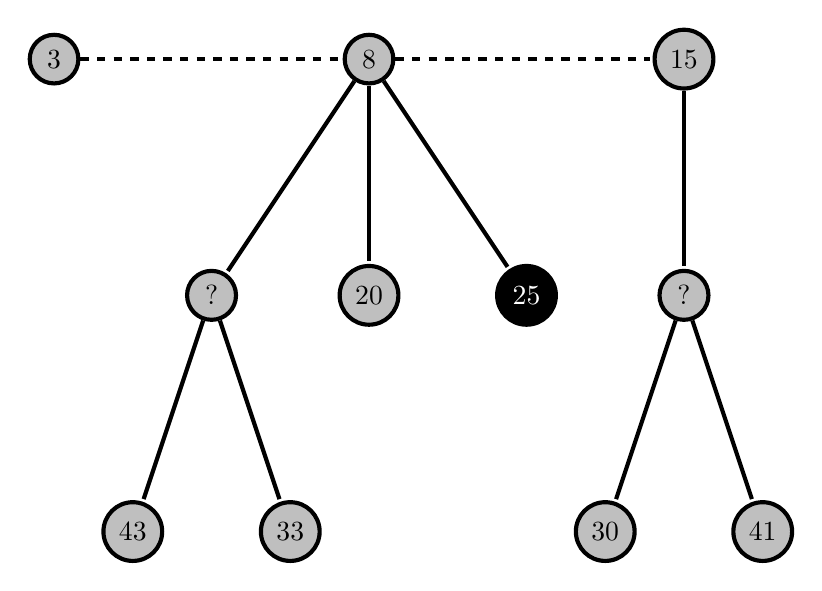
\begin{tikzpicture}[-,>=stealth,shorten >=1pt,auto,
      main node/.style={circle,draw}, line width=1.5pt]
  \node[main node,fill=lightgray] (a) at (-1,0) {3};
  \node[main node,fill=lightgray] (b) at (3,0) {8};
  \node[main node,fill=lightgray] (c) at (7,0) {15};
  \node[main node,fill=lightgray] (d) at (1,-3) {?};
  \node[main node,fill=lightgray] (e) at (3,-3) {20};
  \node[main node,fill=black,text=white] (f) at (5,-3) {25};
  \node[main node,fill=lightgray] (g) at (7,-3) {?};
  \node[main node,fill=lightgray] (h) at (2,-6) {33};
  \node[main node,fill=lightgray] (j) at (0,-6) {43};
  \node[main node,fill=lightgray] (i) at (6,-6) {30};
  \node[main node,fill=lightgray] (k) at (8,-6) {41};
  \path[every node/.style={font=\small}]
  (a) edge[dashed] (b)
  (b) edge[dashed] (c)
  (b) edge (d)
  (b) edge (e)
  (b) edge (f)
  (c) edge (g)
  (d) edge (h)
  (g) edge (i)
  (d) edge (j)
  (g) edge (k)
  ;
  \end{tikzpicture}
\end{center}
\fleresvar
\mulighederstart
\svar 3
\svar 5
\svar 12 \korrekt
\svar 18 \korrekt
\svar 32 \korrekt
\svar 42
\mulighederslut
\forklaring{For knuden til venstre skal værdien ligge mellem 8 og 33 (den laveste værdi i et barn), dvs. 12, 18 og 32 er mulige. For knuden til højre skal værdien ligge mellem 15 og 30, hvilket ikke giver yderligere muligheder.}


\spoergsmaal{Længste fælles delsekvens}
Hvilke af disse strenge er længste fælles delsekvenser (eng.~\emph{longest common subsequences}) af strengene \texttt{AABCBDAA} og \texttt{BACDBAAB}?
\fleresvar

\mulighederstart
\svar \texttt{ABCBA}
\svar \texttt{ABCAB}
\svar \texttt{ACBAA}\korrekt
\svar \texttt{ACDAA}\korrekt
\svar \texttt{BBDAA}
\svar \texttt{BBCDA}
\svar \texttt{BCBAA}\korrekt
\svar \texttt{BCDAA}\korrekt
\mulighederslut

%Longest Common Subsequence returned by std. algo: ACBAA
%Alternative LCS: BCBAA, BCDAA, ACDAA

\forklaring{Håndkørsel af algoritmen til længste fælles delsekvens i CLRS sektion 15.4 giver denne dynamisk programmeringstabel:
\begin{center}
\begin{tabular}{c|c|c|c|c|c|c|c|c|c||}
    &   & B & A & C & D & B & A & A & B\\
    \hline
     & 0 & 0 & 0 & 0 & 0 & 0 & 0 & 0 & 0\\
     \hline
    A & 0 & $\uparrow0$ & $\nwarrow1$ & $\leftarrow1$ & $\leftarrow1$ & $\leftarrow1$ & $\nwarrow1$ & $\nwarrow1$ & $\leftarrow1$ \\
    A & 0 & $\uparrow0$ & $\nwarrow1$ & $\uparrow1$ & $\uparrow1$ & $\uparrow1$ & $\nwarrow2$ & $\nwarrow2$ & $\leftarrow2$ \\
    B & 0 & $\nwarrow1$ & $\uparrow1^*$ & $\uparrow1$ & $\uparrow1$ & $\nwarrow2$ & $\uparrow2$ & $\uparrow2$ & $\nwarrow3$ \\
    C & 0 & $\uparrow1$ & $\uparrow1$ & $\nwarrow2$ & $\leftarrow2$ & $\uparrow2$ & $\uparrow2$ & $\uparrow2$ & $\uparrow3$ \\
    B & 0 & $\nwarrow1$ & $\uparrow1$ & $\uparrow2$ & $\uparrow2$ & $\nwarrow3$ & $\leftarrow3$ & $\leftarrow3$ & $\nwarrow3$ \\
    D & 0 & $\uparrow1$ & $\uparrow1$ & $\uparrow2$ & $\nwarrow3$ & $\uparrow3^*$ & $\uparrow3$ & $\uparrow3$ & $\uparrow3$ \\
    A & 0 & $\uparrow1$ & $\nwarrow2$ & $\uparrow2$ & $\uparrow3$ & $\uparrow3$ & $\nwarrow4$ & $\nwarrow4$ & $\leftarrow4$ \\
    A & 0 & $\uparrow1$ & $\nwarrow2$ & $\uparrow2$ & $\uparrow3$ & $\uparrow3$ & $\nwarrow4$ & $\nwarrow5$ & $\leftarrow5$ \\
    \hline
\end{tabular}
\end{center}
To steder (markeret med $^*$) er der mulighed for at ``vælge retning'' på to måder, hvilket giver fire korrekte længste fælles delsekvenser af længde 5.
De øvrige valgmuligheder er ikke fælles delsekvenser.
}


\spoergsmaal{Dynamisk programmering}
Vi betragter algoritmen til længste fælles delsekvens (eng.~\emph{longest common subsequence}) i CLRS sektion 15.4.
Antag at tabellen $b$ efter kørsel på to strenge ser ud som nedenfor.
Hvad er længden af en længste fælles delsekvens?
%X = "ABRAMS"
%Y = "RAMADAN"
\begin{center}
\begin{tabular}{|c|c|c|c|c|c|c|}
    \hline
    $\uparrow$ & $\nwarrow$ & $\leftarrow$ & $\nwarrow$ & $\leftarrow$ & $\nwarrow$ & $\leftarrow$ \\
    \hline
    $\uparrow$ & $\uparrow$ & $\uparrow$ & $\uparrow$ & $\uparrow$ & $\uparrow$ & $\uparrow$ \\
    \hline
    $\nwarrow$ & $\uparrow$ & $\uparrow$ & $\uparrow$ & $\uparrow$ & $\uparrow$ & $\uparrow$ \\
    \hline
    $\uparrow$ & $\nwarrow$ & $\leftarrow$ & $\nwarrow$ & $\leftarrow$ & $\nwarrow$ & $\leftarrow$ \\
    \hline
    $\uparrow$ & $\uparrow$ & $\nwarrow$ & $\leftarrow$ & $\leftarrow$ & $\leftarrow$ & $\leftarrow$ \\
    \hline
    $\uparrow$ & $\uparrow$ & $\uparrow$ & $\uparrow$ & $\uparrow$ & $\uparrow$ & $\uparrow$ \\
    \hline
\end{tabular}
\end{center}
\etsvar
\mulighederstart
\svar 1
\svar 2
\svar 3\korrekt
\svar 4
\svar 5
\svar 6
\mulighederslut
\forklaring{Den længste fælles delsekvens kan findes ved at følge pilene fra nederste højre hjørne: $\uparrow$, $\leftarrow$, $\leftarrow$, $\leftarrow$, $\leftarrow$, $\nwarrow$, $\nwarrow$, $\nwarrow$.
Den længste fælles delsekvens svarer til de tre $\nwarrow$.}


\spoergsmaal{Søgetræer}
Vi betragter et binært søgetræ der indeholder $n$ forskellige nøgler, $x_1,\dots,x_n$, og har højde~$h$.
Hvad kan man med sikkerhed sige (uden at vide andet om træet) om tiden for at søge efter nøglerne $x_1,\dots,x_n$?
\fleresvar
\mulighederstart
\svar Tiden er $\Theta(\log n)$ for den værste nøgle $x_i$.
\svar Tiden er $\Theta(h)$ for den værste nøgle $x_i$. \korrekt
\svar Tiden er $\Theta(n)$  for den værste nøgle $x_i$.
\svar Tiden er $O(\log n)$ i gennemsnit over $x_1,\dots,x_n$.
\svar Tiden er $O(h)$ i gennemsnit over $x_1,\dots,x_n$. \korrekt
\svar Tiden er $O(n)$ i gennemsnit over $x_1,\dots,x_n$. \korrekt
\mulighederslut
\forklaring{Tiden er $\Theta(h)$ i værste fald hvor der søges efter en nøgle $x_i$ i dybde $h$.
Det medfører at gennemsnitstiden er $O(h)$.
Da træet ikke nødvendigvis er balanceret kan højden være større end $O(\log n)$ (også i gennemsnit), så tiden er ikke $O(\log n)$. Tilsvarende kan højden være $o(n)$, så tiden er ikke $\Omega(n)$. }


\spoergsmaal{Rød-sorte søgetræer}
Betragt et rød-sort binært søgetræ $T$, som beskrevet i CLRS kapitel 13, hvor bladene er udeladt og to indre knuder er uspecificerede:
\begin{center}
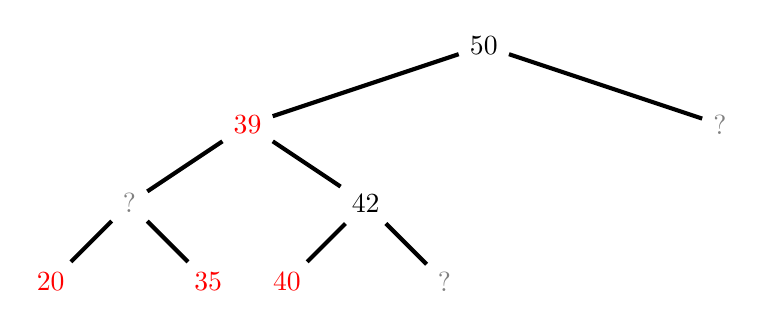
\begin{tikzpicture}[-,>=stealth,level/.style={sibling distance = 6cm/#1,
    level distance = 1cm}, line width=1.5pt] 
  \node [black] {50}
      child{ node [red] {39} 
              child{ node [gray] {?} 
                  child{ node [red] {20} }
                  child{ node [red] {35}}
              }
              child{ node [black] {42}
                              child{ node [red] {40}}
                              child{ node [gray] {?}}
              }                            
      }
      child{ node [gray] {?}
          }
  ; 
  \end{tikzpicture}  
\end{center}
\noindent
Hvilke knuder er mulige for \emph{mindst én} af de tre uspecificerede positioner, hvis træet skal overholde de rødsorte egenskaber?
\fleresvar
\mulighederstart
\svar En rød knude med nøglen 25.
\svar En sort knude med nøglen 32. \korrekt
\svar En sort knude med nøglen 38.
\svar En rød knude med nøglen 45. \korrekt
\svar En sort knude med nøglen 55. \korrekt
\svar En rød knude med nøglen 60.
\svar En sort knude med nøglen 70. \korrekt
\mulighederslut
\forklaring{ Der skal være lige mange sorte knuder på alle stier fra roden til et blad, dvs.~der skal være to på hver sti. Det betyder at knuderne, fra venstre til højre, har farverne sort, rød, sort. Nøglerne skal desuden placeres således, at søgetræ-invarianten opretholdes.}


\spoergsmaal{Mindste udspændende træ}
Betragt denne vægtede graf:
\begin{center}
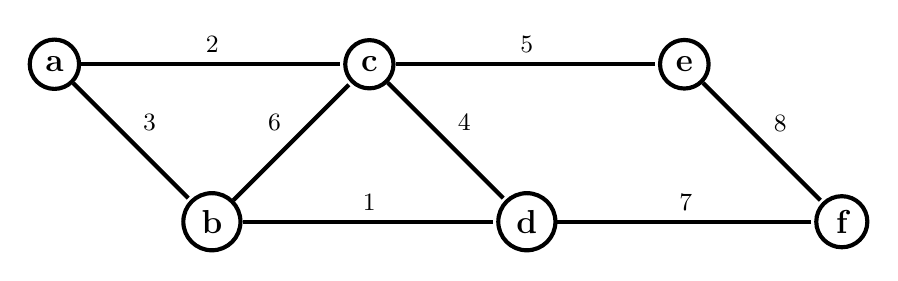
\begin{tikzpicture}[-,>=stealth,shorten >=1pt,auto,
  main node/.style={circle,draw,font=\large\bfseries}, line width=1.5pt]
\node[main node] (a) at (0,2) {a};
\node[main node] (b) at (2,0) {b};
\node[main node] (c) at (4,2) {c};
\node[main node] (d) at (6,0) {d};
\node[main node] (e) at (8,2) {e};
\node[main node] (f) at (10,0) {f};

\path[every node/.style={font=\small}]
(a) edge node {3} (b)
(a) edge node {2} (c)
(b) edge node {1} (d)
(c) edge node {4} (d)
(c) edge node {5} (e)
(d) edge node {7} (f)
(e) edge node {8} (f)
(b) edge node {6} (c);
\end{tikzpicture}
\end{center}
Det mindste udspændende træ (eng.~\emph{minimum spanning tree}) er unikt. Hvilke kanter indgår i det mindste udspændende træ?
\fleresvar
\mulighederstart
\svar \{a,b\} \korrekt
\svar \{a,c\} \korrekt
\svar \{b,c\}
\svar \{b,d\} \korrekt
\svar \{c,d\}
\svar \{c,e\} \korrekt
\svar \{d,f\} \korrekt
\svar \{e,f\} 
\mulighederslut
\forklaring{Ved at anvende fx Prim's algoritme ses at de markerede kanter indgår i MST'et.}

\spoergsmaal{Mindste udspændende træ}
Betragt en vægtet, uorienteret graf med knudemængde $V = \{1,2,\ldots,n\}$ og kanter mellem alle par af knuder.
Kanten fra knude $u$ til knude $v$ har vægt $w(u,v) = |u-v|$.
Nedenfor vises grafen for tilfældet $n=4$.

\begin{center}
  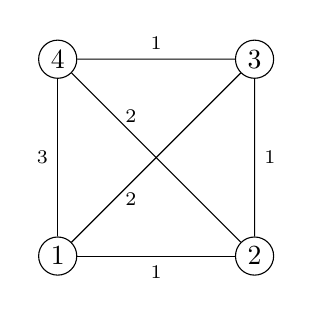
\begin{tikzpicture}[scale=1.25, 
    vertex/.style={circle, draw, fill=white, inner sep=2pt},
    every edge/.style={draw}]
  % Define positions of vertices
  \node[vertex] (1) at (0,0) {1};
  \node[vertex] (2) at (2,0) {2};
  \node[vertex] (3) at (2,2) {3};
  \node[vertex] (4) at (0,2) {4};
  % Draw edges with weights (no circles on weights)
  \draw (1) -- (2) node[midway, below] {\scriptsize $1$};
  \draw (1) -- (3) node[pos=0.35, below] {\scriptsize $2$};
  \draw (1) -- (4) node[midway, left] {\scriptsize $3$};
  \draw (2) -- (3) node[midway, right] {\scriptsize $1$};
  \draw (4) -- (2) node[pos=0.35, above] {\scriptsize $2$};
  \draw (3) -- (4) node[midway, above] {\scriptsize $1$};
\end{tikzpicture}
\end{center}

Hvad er vægten af det mindste udspændende træ, som funktion af $n$?
\etsvar
\mulighederstart
\svar $\Theta(\sqrt{n})$
\svar $\Theta(n)$ \korrekt
\svar $\Theta(n \log n)$
\svar $\Theta(n^2)$
\svar $\Theta(2^n)$
\mulighederslut

\forklaring{
For at finde et mindste udspændende træ (MST) skal vi vælge $n-1$ kanter, så alle $n$ knuder forbindes uden at danne en cykel, og summen af vægterne er mindst mulig.
En strategi er at forbinde knuderne i rækkefølge: $1$ med $2$, $2$ med $3$, osv., altså bruge kanterne $\{1,2\}$, $\{2,3\}$, $\{3,4\}$, ..., $\{n-1,n\}$. Hver af disse kanter har vægt $1$, og der er $n-1$ af dem, så den samlede vægt bliver $M_n = n-1$.
Da ingen vægte er mindre end 1 er dette optimalt.
Dermed vokser vægten af MST som $\Theta(n)$.%, da vægten vokser lineært med $n$.
}
%For an integer $n >0$, let $K_n = (V_n,E_n)$ be the complete graph on the vertex-set $V = \{1,2,\ldots,n\}$. Let $W_n : E_n \to \mathbb{R}$
%be defined by
%$W_n(e) = |i-j|$ where $e = \{i,j\} \in E_n$.
%Denote by $M_n$ the weight of a minimum spanning tree for $K_n$ with respect to $W_n$.
%Which of the following is true?
%\mulighederstart
%\svar $M_n = \Theta(n)$ \korrekt
%\svar $M_n = \Theta(n^2)$
%\svar $M_n = \Theta(\sqrt{n})$
%\svar $M_n = \Theta(2^n)$
%\svar $M_n = \Theta(n \log n)$
%\mulighederslut


\spoergsmaal{Korteste veje}
Betragt en vægtet, orienteret graf med knudemængde $V = \{1,2,\ldots,n\}$ og én kant mellem alle par af knuder.
For knuder $u$ og $v$ med $u<v$ er der en kant fra $u$ til $v$ med vægt $w(u,v) = v$, men ikke nogen kant fra $v$ til $u$.
Nedenfor vises grafen for tilfældet $n=5$.
%Fastlæg et heltal $n >0$, 
%og betragt mængden af knuder $V = \{1,2,\ldots,n\}$.
%For alle forskellige $i,j \in V$,
%definér vægten af den rettede kant $e = (i,j)$ som $W(e) = j$.
%Der er ikke nogen kant $(j,i)$ når $j>i$.
%Nedenfor ses som eksempel grafen for $n=5$.
%
\begin{center}
\begin{tikzpicture}[
    >=Stealth,
    vertex/.style={circle, draw, minimum size=1cm},
    edge/.style={->, thick}
  ]
  % Nodes
  \node[vertex] (1) at (0,0) {1};
  \node[vertex] (2) at (2,1.5) {2};
  \node[vertex] (3) at (4,0) {3};
  \node[vertex] (4) at (6,1.5) {4};
  \node[vertex] (5) at (8,0) {5};

  % Edges with straight lines
  \draw[edge] (1) -- node[midway, sloped, above] {2} (2);
  \draw[edge] (1) -- node[midway, sloped, below] {3} (3);
  \draw[edge] (1) to[bend right=30] node[midway, below] {5} (5); % curved
  \draw[edge] (1) to[bend left=55] node[midway, above] {4} (4); % curved

  \draw[edge] (2) to[bend right=15] node[midway, above] {3} (3); % curved
  \draw[edge] (2) -- node[midway, sloped, above] {4} (4);
  \draw[edge] (2) to[bend left=55] node[midway, above] {5} (5); % curved

  \draw[edge] (3) to[bend right=15] node[midway, above] {4} (4); % curved
  \draw[edge] (3) -- node[midway, sloped, below] {5} (5);

  \draw[edge] (4) -- node[midway, sloped, above] {5} (5);

\end{tikzpicture}
\end{center}
%
Betegn med $\delta(u,v)$ længden af den korteste vej i grafen fra $u$ til $v$.
Hvad er den største afstand fra knude $1$ til en anden knude i grafen, dvs.~hvad er $\max_v(\delta(1,v))$?
\etsvar
%Fix an integer $n >0$, 
%and consider the vertex-set $V = \{1,2,\ldots,n\}$.
%For every distinct $i,j \in V$,
%define the weight of the directed edge $e = (i,j)$ by $W(e) = j^2$.
%Denote by $D(i,j)$ the shortest path distance with respect to $W$ between $i$ and $j$.
%What is the maximum distance from the vertex $1$?
\mulighederstart
\svar $\lceil n/2\rceil$
\itxsvar{ceiling(n/2)}
\svar $n$ \korrekt
\svar $\lceil 3n/2\rceil$
\itxsvar{ceiling(3n/2)}
\svar $2n$
\mulighederslut

\forklaring{Den korteste vej fra $1$ til $j$ er altid den direkte kant, hvilket kan vises ved induktion i $n$. Dvs.~$\delta(1,j) = j$ som er højst $n$. Alternativt kan alle andre muligheder udelukkes ved at se på eksemplet ovenfor.}


\spoergsmaal{Bellman-Ford}
Betragt nedenstående orienterede graf $G$, med en uspecificeret vægt $x$:
\begin{center}
\begin{tikzpicture}[
    >=Stealth,
    vertex/.style={circle, draw, minimum size=1cm},
    edge/.style={->, thick}
  ]
  % Nodes
  \node[vertex] (1) at (0,0) {1};
  \node[vertex] (2) at (2,1.5) {2};
  \node[vertex] (3) at (4,0) {3};
  \node[vertex] (4) at (6,1.5) {4};
  \node[vertex] (5) at (8,0) {5};

  % Edges with straight lines
  \draw[edge] (1) -- node[midway, sloped, above] {-1} (2);
  \draw[edge] (3) -- node[midway, sloped, below] {4} (1);
  \draw[edge] (1) to[bend right=25] node[midway, below] {6} (5); % curved

  \draw[edge] (2) to[bend right=0, sloped] node[midway, above] {$x$} (3); % curved
  \draw[edge] (4) -- node[midway, sloped, above] {2} (2);

  \draw[edge] (3) to[bend right=0, sloped] node[midway, above] {-3} (4); % curved
  \draw[edge] (3) -- node[midway, sloped, below] {0} (5);

  \draw[edge] (5) -- node[midway, sloped, above] {3} (4);

\end{tikzpicture}
\end{center}

Lad $w_x$ betegne $G$'s vægtvektor. 
For hvilke værdier af $x$ returnerer $\proc{Bellman-Ford}(G, w_x, 1)$ fra CLRS sektion 22.1 værdien {\sc True}?
\fleresvar
\mulighederstart
\svar $x=2$\korrekt
\svar $x=1$\korrekt
\svar $x=0$
\svar $x=-1$
\svar $x=-2$
\mulighederslut
\forklaring{Hvis $x\leq 0$ er der en negativ cykel mellem knuderne 2, 3, 4, der kan nås fra knude~1, så $\proc{Bellman-Ford}$ returnerer {\sc False}. Hvis $x\geq 1$ findes der ikke nogen negativ cykel i grafen så $\proc{Bellman-Ford}$ returnerer {\sc True}.}


\spoergsmaal{Valg af algoritme}
Givet to usorterede arrays $A[1:n]$ og $B[1:m]$ med henholdsvis $n$ og $m$ elementer ønsker vi at finde antal elementer der optræder i begge arrays.
Ingen af de to arrays har elementer, der gentager sig, dvs.~de indeholder henholdsvis $n$ og $m$ forskellige elementer.
Lad $T$ være et rød-sort søgetræ. Vi betragter to mulige algoritmer:
\begin{codebox}
\Procname{$\proc{Intersection-BruteForce}(A, B, n, m)$}
\li $count \gets 0$
\li \For $i \gets 1$ \To $n$ 
\li \Do
        \For $j \gets 1$ \To $m$
\li     \Do
            \If $A[i] = B[j]$ 
\li         \Then $count \gets count + 1$
            \End
        \End
    \End
\li \Return $count$
\end{codebox}
\begin{codebox}
\Procname{$\proc{Intersection-Tree}(A, B, n, m)$}
\li $T.root \gets \proc{nil}$ \Comment{$T$ er nu et tomt søgetræ}
\li \For $j \gets 1$ \To $m$
\li \Do \text{Lad $z$ være en ny, tom RB-træknude}
\li $z.key \gets B[j]$
\li $\proc{RB-Insert}(T, z)$ \End
\li $count \gets 0$
\li \For $i \gets 1$ \To $n$
\li \Do
        \If $\proc{Tree-Search}(T, A[i]) \neq \proc{nil}$
\li     \Then $count \gets count + 1$
     \End
    \End
\li \Return $count$
\end{codebox}
Hvilken algoritme der er asymptotisk hurtigst afhænger af forholdet mellem parametrene $m$ og $n$.
For hvilke af nedenstående valg af $m$ er $\proc{Intersection-BruteForce}$ asymptotisk mindst lige så hurtig som $\proc{Intersection-Tree}$?
\fleresvar
\mulighederstart
\svar $m = \Theta(1)$\korrekt
\svar $m = \Theta(n)$
\svar $m = \Theta(n^2)$
\svar $m = \Theta(2^n)$\korrekt
\mulighederslut
\forklaring{Køretiden for $\proc{Intersection-BruteForce}$ er $\Theta(nm)$, mens køretiden for proceduren $\proc{Intersection-Tree}$ er $\Theta(m\log m + n\log m)$.
Ved at indsætte de fire valg af $m$ i køretiderne får vi at køretider: 1.~$\Theta(n)$ for begge algoritmer, 2.~$\Theta(n^2)$ henholdsvis $\Theta(n\log n)$, 3.~$\Theta(n^3)$ henholdsvis $\Theta(n^2\log n)$, 4.~$\Theta(n\cdot 2^n)$ for begge algoritmer.
}

\spoergsmaal{Matrixkæde-multiplikation}
Algoritmen {\sc Matrix-Chain-Order}$(p,n)$ fra CLRS 14.2 returnerer to arrays $m$ og $s$.
Nedenfor ses et array $s[1:n-1, 2:n]$ returneret af {\sc Matrix-Chain-Order}$(p,n)$ for et produkt af $n=6$ matricer $A_1\cdots A_6$ med dimensioner angivet i $p$.
\medskip

\begin{tabular}{c|ccccc}
$i \backslash j$ & 2 & 3 & 4 & 5 & 6 \\
\hline
1 & 1 & 1 & 3 & 4 & 4 \\
2 &   & 2 & 3 & 4 & 4 \\
3 &   &   & 3 & 4 & 4 \\
4 &   &   &   & 4 & 5 \\
5 &   &   &   &   & 5 \\
\end{tabular}

\medskip\noindent
Angiv måden at sætte parenteser på ifølge tabellen.
\etsvar
%
\mulighederstart
\svar $((A_1( A_2A_3))A_4)(A_5A_6)$.\korrekt
\svar $(A_1(A_2 A_3))((A_4 A_5)A_6)$
\svar $A_1((A_2(A_3A_4))(A_5 A_6))$ 
\svar $((((A_1 A_2)A_3)A_4)A_5)A_6$.
\svar $(A_1(A_2 A_3))(A_4(A_5 A_6))$.
\mulighederslut
\forklaring{Vi håndkører algoritmen {\sc Print-Optimal-Parens}$(s,1,n)$. Da $s[1,6]=4$ er de yderste parenteser $(A_1A_2A_3A_4)(A_5A_6)$.
Dette passer kun med mulighed 1.}


\spoergsmaal{Disjunkte mængder}
Vi betragter trærepræsentationer af disjunkte mængder (eng.~\emph{disjoint sets}), som beskrevet i CLRS sektion 19.3, ved brug af heuristikken \emph{union by rank} uden brug af stiforkortning.
En algoritme laver $n$ kald til {\sc Make-Set}, $n^2$ kald til {\sc Find-Set}, og $n-1$ kald til {\sc Union}.
Hvad er den bedste (mindste) af følgende tidsgrænser som vi kan garantere for den samlede tid disse operationer tager?
\etsvar
\mulighederstart
\svar Tiden er $O(n)$
\svar Tiden er $O(n \log n)$
\svar Tiden er $O(n^2)$
\svar Tiden er $O(n^2 \log n)$ \korrekt
\svar Tiden er $O(n^3)$
\svar Tiden er $O(n^3 \log n)$
\mulighederslut
\forklaring{ Tiden er domineret af de $n^2$ {\sc Find-Set} operationer der hver har en tidsgrænse på $O(\log n)$.}


\multiplechoiceslut

\newpage

\section*{Skriftlige opgaver}\label{sec:written}

{\bf Skriftlige opgaver} afleveres som et Word dokument i ITX systemet.
Der er mulighed for at tegne og skrive på tablet, og indsætte i dokumentet.
\begin{itemize}
    \item Brug \emph{én side til hvert delspørgsmål, i samme rækkefølge som i opgavesættet.} 
    \item Delspørgsmålets nummer/bogstav (fx 19 eller 20.a) skal fremgå.
\end{itemize}



\section{Splejse reb (9\%)}

Vi betragter en multi-mængde $A$ af positive hele tal, som repræsenterer længder af reb vi har til rådighed.
Vi kan nu splejse to reb sammen, og prisen for dette er summen af længderne.
Altså kan vi vælge to tal $x,y\in A$.
At \emph{splejse} $x$ og $y$ betyder at vi opdaterer $A$ til $(A\setminus\{x,y\})\cup\{x+y\}$.
Omkostningen for dette er $x+y$.
Bemærk at $A$ er en multi-mængde, hvilket betyder at $A$ kan indeholder flere elementer med samme værdi, og når vi fjerner $x$, så fjerner vi kun ét element med værdien $x$ (og tilsvarende for $y$).
Vi ønsker at splejse indtil $A$ kun indeholder én værdi, og så den totale omkostning er mindst muligt.
Vi repræsenterer $A$ med et array.

\medskip

\textbf{Eksempel:}
$A=\langle 3,1,7,2\rangle$.
Vi splejser $1$ og $2$ med omkostning $3$ og har $A=\langle 3,7,3\rangle$.
Vi splejser $3$ og $7$ med omkostning $10$ og har $A=\langle 3,10\rangle$.
Vi splejser $3$ og $10$ med omkostning $13$ og har $A=\langle 13\rangle$.
Den totale omkostning ved denne splejsesekvens er $3+10+13=26$.
Bemærk at denne splejsesekvens \emph{ikke} er optimal, da det er muligt at opnå en samlet omkostning på mindre end $26$.

\punkt{a)}
{
Angiv den optimale splejsesekvens og den totale omkostning for $A=\langle 3,1,7,2\rangle$. Det er ikke nødvendigt at bevise at sekvensen er optimal.
}

\forklaring{Vi splejser $1,2$, så $3,3$, så $6,7$, og får en samlet omkostning på $3+6+13=22$.}

\punkt{b)}
{
Beskriv en effektiv algoritme som udregner den mindst mulige totale omkostning på at splejse indtil $A$ kun indeholder én værdi.
}

\forklaring{
Vi bruger en grådig algoritme der hele tiden splejser de to mindste værdier i~$A$.
Dette giver den mindst mulige totale omkostning ved et argument ligesom beviset for optimaliteten af Huffman-koder.
}

\punkt{c)}
{
Forklar hvordan algoritmen fra del b), eller en forbedret algoritme, kan implementeres så køretiden er $O(n\log n)$, hvor $n$ er størrelsen af $A$ til at begynde med.
}

\forklaring{
Vi repræsenterer $A$ som en min-hob, så vi kan fjerne de mindste elementer og lægge nye elementer ind i $O(\log n)$ tid.
Derved bliver den totale køretid $O(n\log n)$, da vi er færdige efter at splejse $n-1$ gange.
}

\newpage
\section{Lange stier i træer (11\%)}%\label{sec:last}

Betragt et binært træ $T$ hvor hver knude har enten to eller ingen børn.
Lad roden være $r$ og for enhver knude $v$, lad $v.left$ og $v.right$ være pointere til hhv.~venstre og højre barn.
Hvis $v$ ikke har nogen børn er $v.left=v.right=NIL$.
I denne opgave ser vi på længder af stier i et træ -- f.eks.~har træet nedenfor en sti af længde 3 fra roden $r$ til bladet $y$ og en sti af længde 5 fra bladet $z$ til bladet $w$.
%
\begin{center}
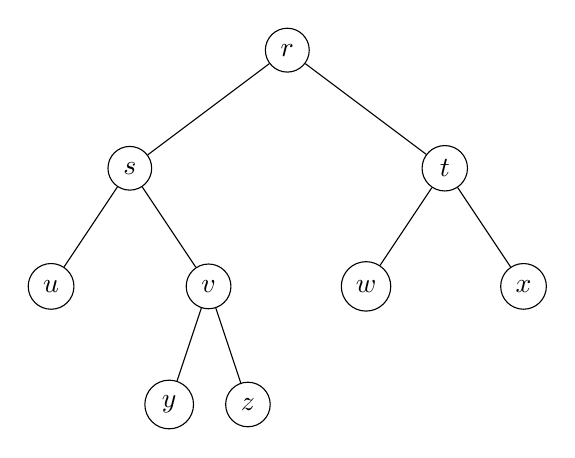
\begin{tikzpicture}[every node/.style={circle, draw},
  level distance=1.5cm,
  level 1/.style={sibling distance=4cm},
  level 2/.style={sibling distance=2cm},
  level 3/.style={sibling distance=1cm}]
\node {$r$}
  child {node {$s$}
    child {node {$u$}
    }
    child {node {$v$}
      child {node {$y$}}
      child {node {$z$}}
    }
  }
  child {node {$t$}
    child {node {$w$}}
    child {node {$x$}}
  };
\end{tikzpicture}
\end{center}


\punkt{a)}
{Vi ønsker at finde den maksimale længde af en sti fra $r$ til et blad.
Længden af en sti er antallet af kanter på stien.
Beskriv en algoritme der løser problemet.
Input til algoritmen er roden $r$.
Du kan evt.~skrive pseudokode, men det er også tilstrækkeligt med en klar og præcis beskrivelse i tekst.
For at få fuldt point skal køretiden være $O(n)$, hvor $n$ er antallet af knuder i $T$.}

\forklaring{Vi kan løse problemet rekursivt, så vi for hver knude $v$ udregner den længste vej fra $v$ til et blad i deltræet med $v$ som rod.
Hvis $v.left==NIL$ returnerer vi $0$, da $v$ selv er et blad.
Ellers løser vi problemet for begge børn og returnerer maksimum af disse plus $1$.
Her er pseudokoden som vi kalder med $v=r$:

\begin{codebox}
\Procname{$\proc{LongestPathToLeaf}(v)$}
\li \If $v.left==NIL$
\li \Then \Return $0$
\End
\li \Return $1+\max\{\proc{LongestPathToLeaf}(v.left),\proc{LongestPathToLeaf}(v.right)\}$
\end{codebox}
}

\punkt{b)}
{Diameteren af $T$ er den maksimale længde af en sti i $T$.
Bevis eller modbevis at en sti af maksimal længde altid starter og slutter i blade.}

\forklaring{Hvis en sti starter eller slutter i en knude som ikke er et blad, kan stien forlænges til et af børnene, da alle knuder som ikke er blade har to børn.
Derfor må den længste sti både starte og slutte i blade.}

\punkt{c)}
{Beskriv en algoritme der udregner diameteren af $T$ og argumentér for dens korrekthed.
Input til algoritmen er roden~$r$.
Du kan evt.~skrive pseudokode, men det er også tilstrækkeligt med en klar og præcis beskrivelse i tekst.
For at få fuldt point skal køretiden være $O(n)$, hvor $n$ er antallet af knuder i $T$.}

\forklaring{Vi udregner først i hver knude $v$ værdien $v.h$ som er længden af den længste sti fra $v$ til et blad under $v$, som i spørgsmål a).
Lad $v.s$ være længden af den længste sti i deltræet med $v$ som rod.
Hvis $v.left=NIL$ sætter vi $v.s=0$.
Ellers er der to tilfælde: Enten er den længste sti indeholdt i et af deltræerne der har et af børnene som rod, eller også går den gennem $v$.
Hvis den går gennem $v$ må den på venstre side gå ned til et blad der er længst under $v.left$ og på højre side gå ned til et blad der er længst under $v.right$.
Derfor kan vi udregne $v.s$ som
\[
v.s=\max\{v.left.s,v.right.s,v.left.h+v.right.h+2\}.
\]
Det kan skrives i pseudokode, hvor vi antager at værdierne $v.h$ er blevet regnet ud før:

\begin{codebox}
\Procname{$\proc{LongestPathInTree}(r)$}
\li \If $r.left==NIL$
\li \Then \Return $0$
\End
\li $ls=\proc{LongestPathInTree}(r.left)$
\li $rs=\proc{LongestPathInTree}(r.right)$
\li \Return $\max\{ls,rs,r.left.h+r.right.h+2\}$
\end{codebox}
}

\newpage
\section{Mindste udspændende træ (8\%)}\label{sec:last}

Lad $(x_1,y_1),\ldots,(x_n,y_n) \in \mathbb{R}^2$ være (forskellige) punkter i planen.
Betegn med $G = (V,E)$ den komplette, uorienterede graf på knuderne $V = \{1,2,\ldots,n\}$. 
Definér vægtfunktionen $W : E \to \mathbb{R}$ som
$$W(\{i,j\}) = \sqrt{(x_i-x_j)^2+(y_i-y_j)^2},$$
dvs.~vægten af kanten $\{i,j\}$ er den Euklidiske afstand mellem punkterne $(x_i,y_i)$ og $(x_j,y_j)$.
Tegningen nedenfor illustrerer en graf $G$ defineret ved 5 numererede punkter placeret på et gitter hvor hvert kvadrat har sidelængde~1.

\begin{center}
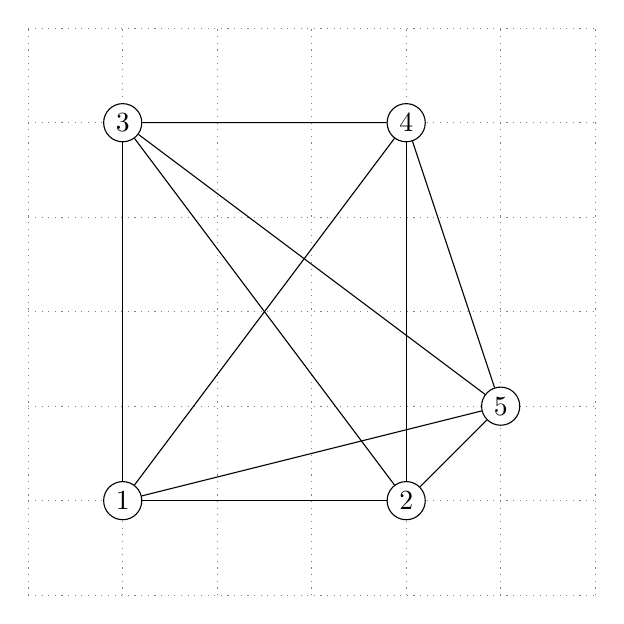
\begin{tikzpicture}[scale=1.2,
    vertex/.style={circle, draw, fill=white, inner sep=2pt},
    every edge/.style={draw}]
  
  % Draw background grid
  \draw[step=1,dotted,gray] (-1,-1) grid (5,5);

  % Define nodes at integer positions with known integer distances
  \node[vertex] (A) at (0,0) {1};
  \node[vertex] (B) at (3,0) {2};
  \node[vertex] (C) at (0,4) {3};
  \node[vertex] (D) at (3,4) {4};
  \node[vertex] (E) at (4,1) {5};

  % Draw all edges of the complete graph (10 edges)
  \draw (A) -- (B);
  \draw (A) -- (C);
  \draw (A) -- (D);
  \draw (A) -- (E);

  \draw (B) -- (C);
  \draw (B) -- (D);
  \draw (B) -- (E);

  \draw (C) -- (D);
  \draw (C) -- (E);

  \draw (D) -- (E);

\end{tikzpicture}
\end{center}

\punkt{a)}
{Hvilke kanter udgør et mindste udspændende træ for grafen $G$ illustreret ovenfor, og hvad er den totale vægt af disse kanter? Et korrekt svar giver fuldt point, men du er velkommen til at argumentere for dit svar.}

\forklaring{Mindste udspændende træ udgøres af kanterne i stien 1--2--5--4--3. Dette kan bekræftes ved for hver kant i stien at betragte snittet der deler grafen dér. Kantlængderne er 3, $\sqrt{2}$, $\sqrt{10}$, 3, dvs.~totalt $6+\sqrt{2}+\sqrt{10}\approx 10.5765$.\medskip}

Betragt nu en vilkårlig graf $G$ med afstande defineret ved en vægtfunktion $W$ som beskrevet ovenfor.
Lad $F \subset E$ være de $n-1$ kanter i et mindste udspændende træ. Vi ønsker at argumentere for at der ikke kan findes par af kanter i $F$, der ``krydser hinanden'' når man tegner grafen i planen.
Mere specifikt, for en kant $e = \{i,j\} \in E$, betegn med $I_e$ det åbne linjestykke, der forbinder punktet $(x_i,y_i)$ og punktet $(x_j,y_j)$:
$$I_e = \{ \lambda (x_i,y_i)+(1-\lambda) (x_j,y_j) : 0 < \lambda < 1\}.$$

\punkt{b)}
{Bevis, at $F$ ikke kan have linjer der krydser hinanden. Mere specifikt, vis at for alle måder at vælge to kanter $e,e' \in F$ så er $I_e \cap I_{e'} = \emptyset$.}

\forklaring{
Antag modstridvis at der findes to kanter $e = \{a,b\}$ og $e' = \{c,d\}$ i $F$, sådan at de krydser hinanden i deres indre, dvs.~$I_e \cap I_{e'} \neq \emptyset$. 
Vi påstår at kanterne kan erstattes med enten kanterne $\{a,c\}$ og $\{b,d\}$ eller med kanterne $\{a,d\}$ og $\{b,c\}$ uden at introducere cykler.
Det kan ses ved at betragte alle måder som $a$, $b$, $c$, $d$ kan være forbundet på i en træstruktur.
Pga.~trekantsuligheden vil dette give et nyt udspændende træ med mindre total vægt, hvilket modsiger antagelsen om, at $F$ er et mindste udspændende træ.
}

%Let $n > 0$ be an integer and let $(x_1,y_1),\ldots,(x_n,y_n) \in \mathbb{R}^2$ be $n$ distinct points in the plane. Denote by $G = (V,E)$ the complete graph on the vertex-set $V = \{1,2,\ldots,n\}$. Define the weight function $W : E \to \mathbb{R}$ by
%$$W(e) = \sqrt{(x_i-x_j)^2+(y_i-y_j)^2}$$
%where $e = \{i,j\} \in E$.
%Fix a minimum spanning tree of $G$ with respect to $W$ and denote by $F \subset E$ the $n-1$ edges in it.
%For an edge $e = \{i,j\} \in E$,
%denote by $I_e$ the open line segment connecting the point $(x_i,y_i)$
%and the point $(x_j,y_j)$:
%$$I_e = \{ \lambda (x_i,y_i)+(1-\lambda) (x_j,y_j) : 0 < \lambda < 1\}.$$
%Prove that for every two distinct edges $e,e' \in F$,
%the intersection $I_e \cap I_{e'}$
%is empty. 

%Sketch: If there is a crossing, there are two ways to flip the edges. Both ways lead to lower total weight by the triangle inequality. One of the two ways does not create cycles. 



\label{page:last}
